\chapter{swash}

%NSLW Equations:Analytical Solutions
%HR Wallingford Internal Workshop
%Dr.D.M.Kelly
%November 2010
%Chapter2: 2.1 Ritter Dam-break Solution

\section{Description}

\subsection{Geometry and mesh}

Size of the model: rectangle (0.8 m x 8 m)

\begin{itemize}
\item Nodes: 3908
\item Elements: 7317
\end{itemize}

The Figure~\ref{fig:swash:mesh} displays the mesh.
\begin{figure}
\centering
\includegraphicsmaybe{[width=.6\textwidth]}{../img/Mesh.png}
\caption{Mesh of the study}\label{fig:swash:mesh}
\end{figure}

The Figure~\ref{fig:swash:bathy} displays the bathymetrie.
\begin{figure}
\centering
\includegraphicsmaybe{[width=.6\textwidth]}{../img/Bathy.png}
\caption{Bathymetry of the study}\label{fig:swash:bathy}
\end{figure}



\subsection{Boundaries}

The Figure~\ref{fig:swash:boundaries} shows the boundaries of the study.
\begin{figure}
\centering
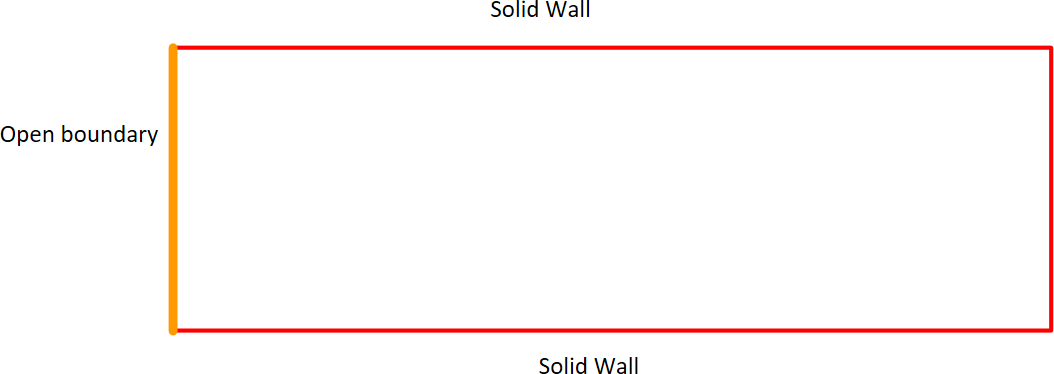
\includegraphics[width=.6\textwidth]{img/boundaries.png}
\caption{Boundaries of the study}\label{fig:swash:boundaries}
\end{figure}

Wave generated for X > 6m:

$H(x) = \frac{1}{20}.x(\frac{0.05}{\cos(atan(0.05))})$

Bottom: No bottom friction

\section{Physical parameters}

Turbulence: Constant viscosity equal to zero


\section{Numerical parameters}

Saint Venant VF Equations
\begin{itemize}
\item Type of element: P1 triangle for h and for velocity
\item Type of advection:   Implicit N scheme on non conservative equation + SUPG decentring on velocities PSI distributive scheme, mass-conservative + modified SUPG on depth
\item Solver:  GMRES
\item Accuracy:  $10^{-4}$
\item Finite volume scheme:  Kinetic order 2
\item Implicitation for depth:   1
\item Implicitation for velocity:  0.6
\end{itemize}

Time data:
\begin{itemize}
\item Time step: 0.001
\item Simulation duration: 12
\end{itemize}

\section{results}


The Figure~\ref{fig:swash:vel} shows the velocity vectors.
\begin{figure}
\centering
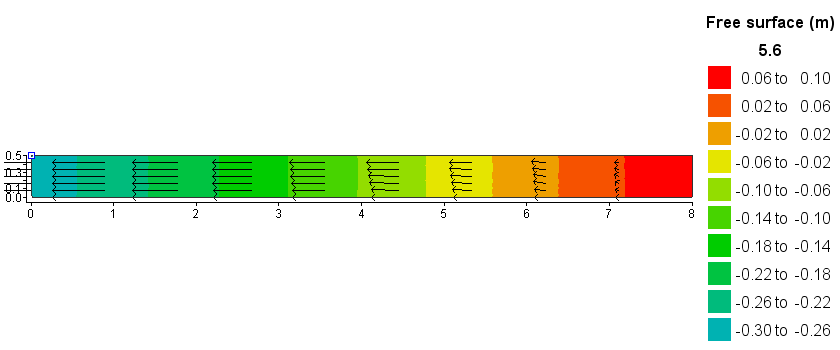
\includegraphics[width=.6\textwidth]{img/vel.png}
\caption{Velocity vectors over the free surface}\label{fig:swash:vel}
\end{figure}

We compare the model and the analytical solution free surface

Comparison Water Free surface
The Figure~\ref{fig:swash:res} shows the comparison for the free surface.
\begin{figure}
\centering
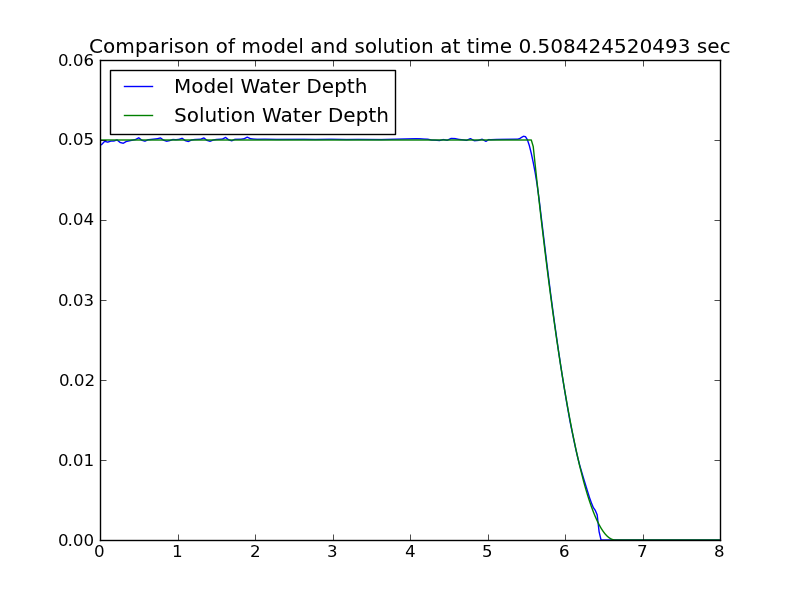
\includegraphics[width=.5\textwidth]{img/res_t0_5.png}
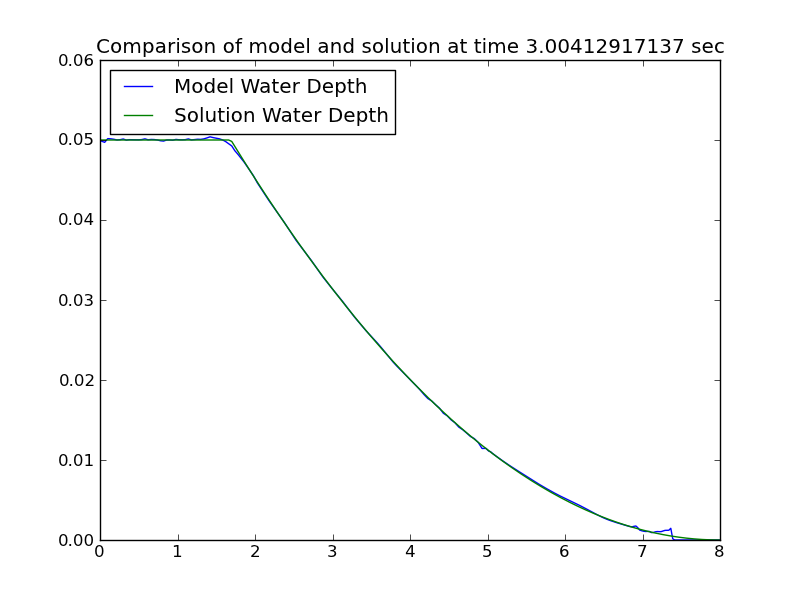
\includegraphics[width=.5\textwidth]{img/res_t3_0.png}
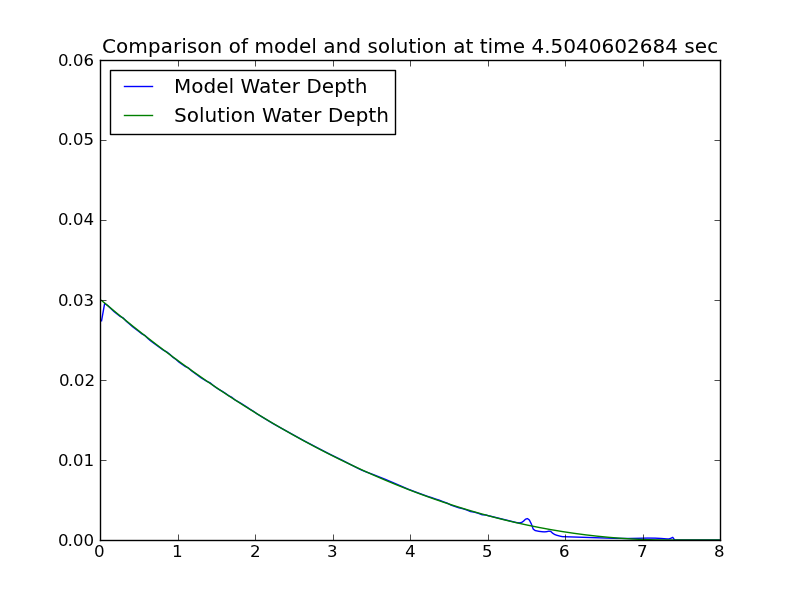
\includegraphics[width=.5\textwidth]{img/res_t4_5.png}
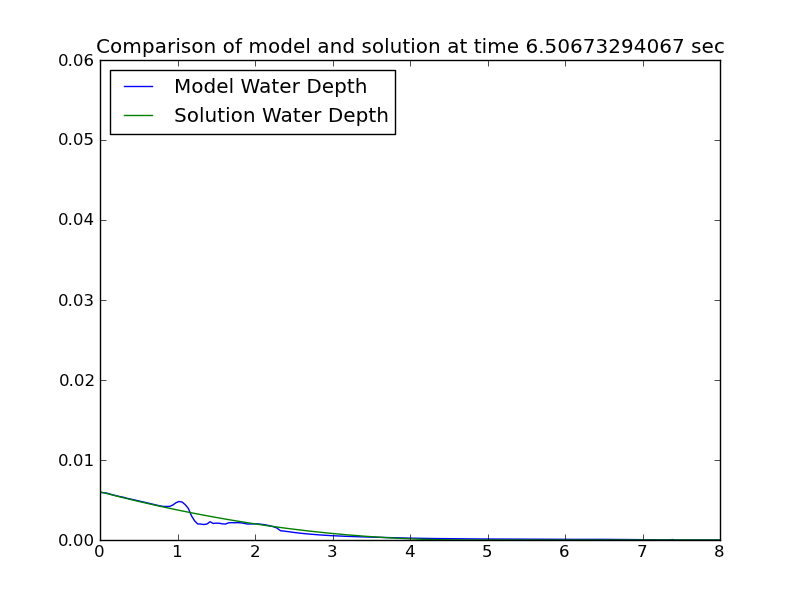
\includegraphics[width=.5\textwidth]{img/res_t6_5.png}
\caption{Comparaison of the results}\label{fig:swash:res}
\end{figure}

Comparison Velocity
The Figure~\ref{fig:swash:res_vel} shows the comparison for the velocity.
\begin{figure}
\centering
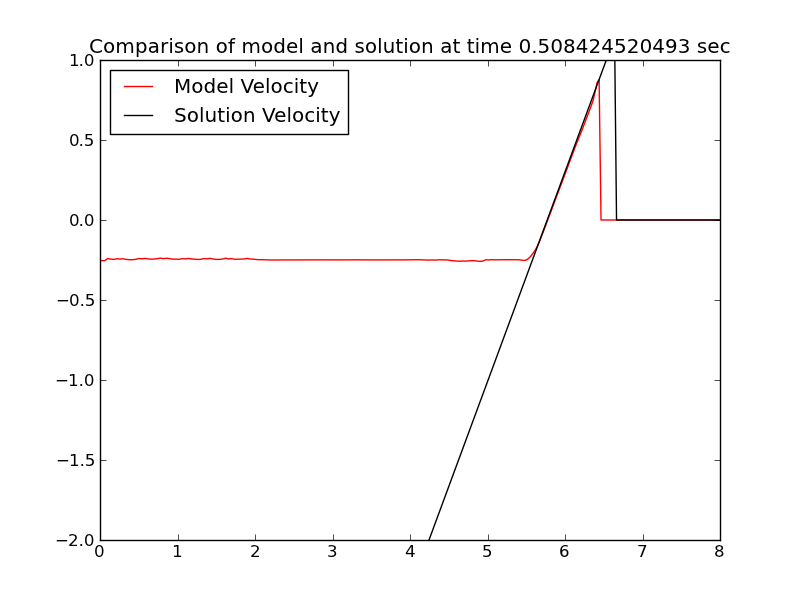
\includegraphics[width=.5\textwidth]{img/res_vel_t0_5.png}
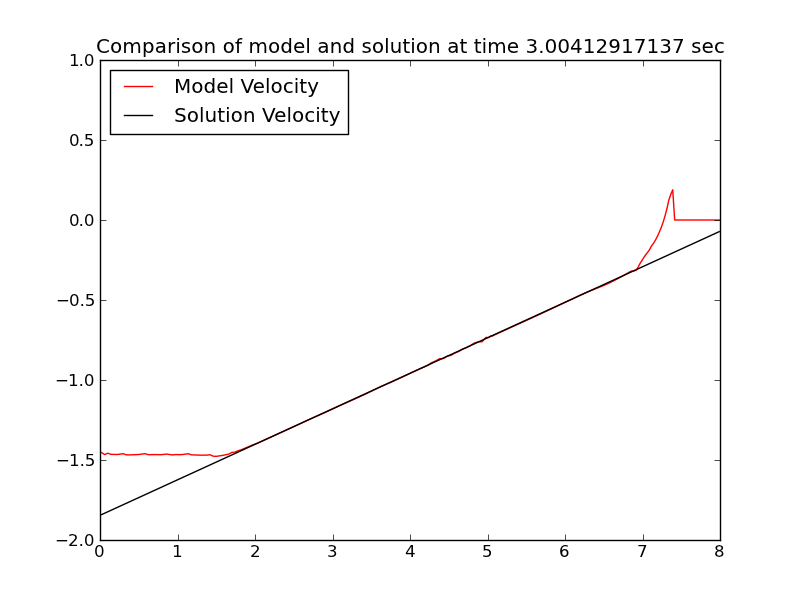
\includegraphics[width=.5\textwidth]{img/res_vel_t3_0.png}
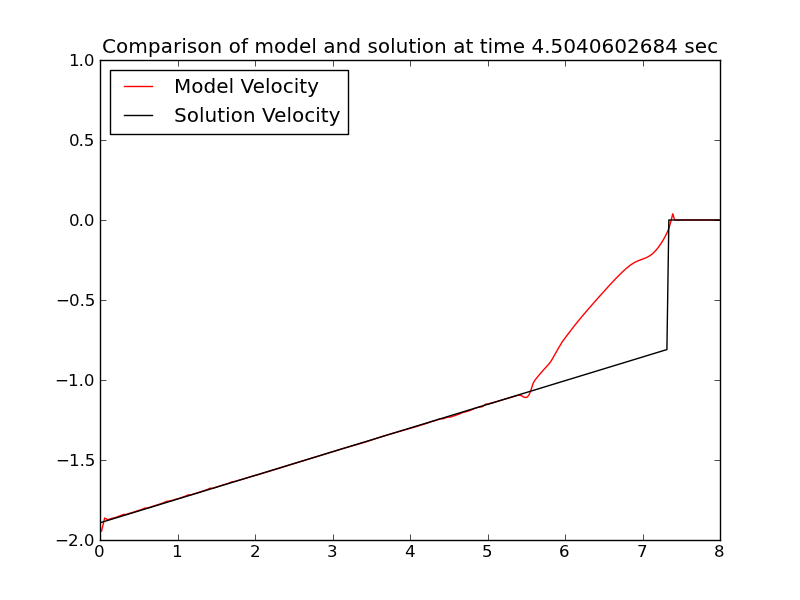
\includegraphics[width=.5\textwidth]{img/res_vel_t4_5.png}
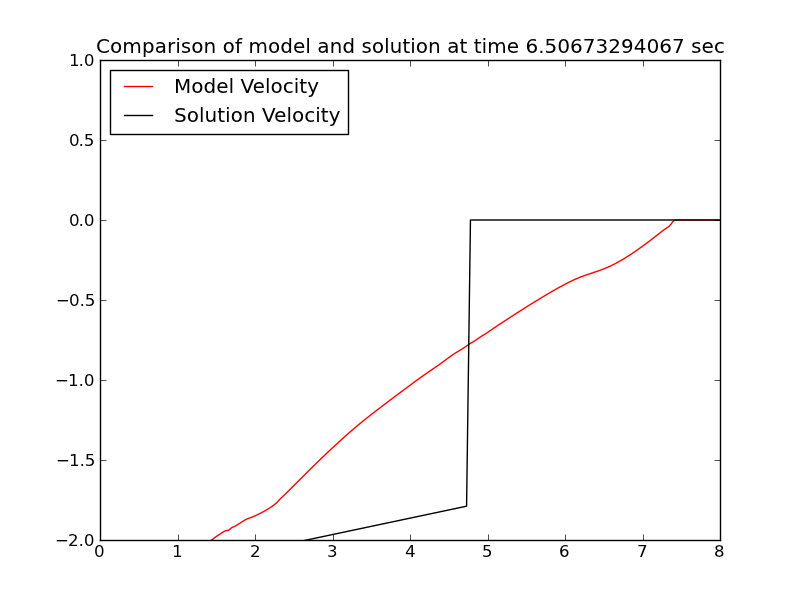
\includegraphics[width=.5\textwidth]{img/res_vel_t6_5.png}
\caption{Comparaison of the results for the veolicty}\label{fig:swash:res_vel}
\end{figure}
